\chapter{Site Works}

\epigraph{In most people’s vocabularies, design means veneer. It’s interior decorating. It’s the fabric of the curtains and the sofa. But to me, nothing could be further from the meaning of design. Design is the fundamental soul of a man-made creation that ends up expressing itself in successive outer layers of the product or service.}{Steve Jobs}

Siteworks encompass the actual construction. Everything we do is immaterial
unless the works on site can be executed.

\section*{Responsibilities}

Any works on site fall under the responsibility of the relevant Section Engineers.
The Project Manager will manage his section\sidenote{A section of the works
is not necessarily defined by area, but it can also be defined by service for example drainage works will normally fall onto one or two section Engineers, whereas another one might be responsible for a Tower.} of the works but ultimately
the owner of a section of the works is the Project or Site Engineer.


\section*{Resource Scheduling}

The Section Engineer is responsible to plan, monitor the execution of the works
and produce daily and weekly reports as required.

\section*{Workflow}

All Section Engineers and as a matter of fact everyone working on the Project
must be familiar with the standards required of the Project by having read the
specification and by having studied the drawings of his section.

On having been allocated a section of the works the Section Engineer needs to
complete the following activities:

\begin{enumerate}
\item \textit{Review Shop Drawings} One needs to take into consideration that
 Shop drawings might not contain the full information required to carry out the works. The Section Engineer must review the drawings carefully, assist if necessary
with comments that will enable further details to be added and that co-ordination
is possible, ceiling heights achievable and shafts workable.

\item Keep a set of drawings for red-marking.
\item Create a Materials Plan.
\item Prepare Material Take-offs.
\item Issue Site Order Releases.
\item Liaise with Main Contractor for Civil works.
\end{enumerate}


In many instances due to Projects peaking at different times, it is quite likely
that an Engineer will be allocated to a Project during a period that the works
are under pressure. This should not really matter, but then it is still the Section
Engineer's responsibility to make sure that the above steps are followed. If he
is replacing someone that has left the Project then if there is a handover report 
one can verify that the information is correct.

\section*{Site Diary}

All Section Engineer's should keep a Site Diary in which to record the day to
day activities of the works. The Site Diary can be invaluable if claims are
lodged and eventually there is arbitration. The minimum information that must
be logged is:

Area and type of works : start date/end date.

Personnel allocation.

Problems encountered.

Key events related to milestones.

In general keep as much information as possible to enable someone - with your
assistance to recreate the events during the construction period.
\begin{marginfigure}
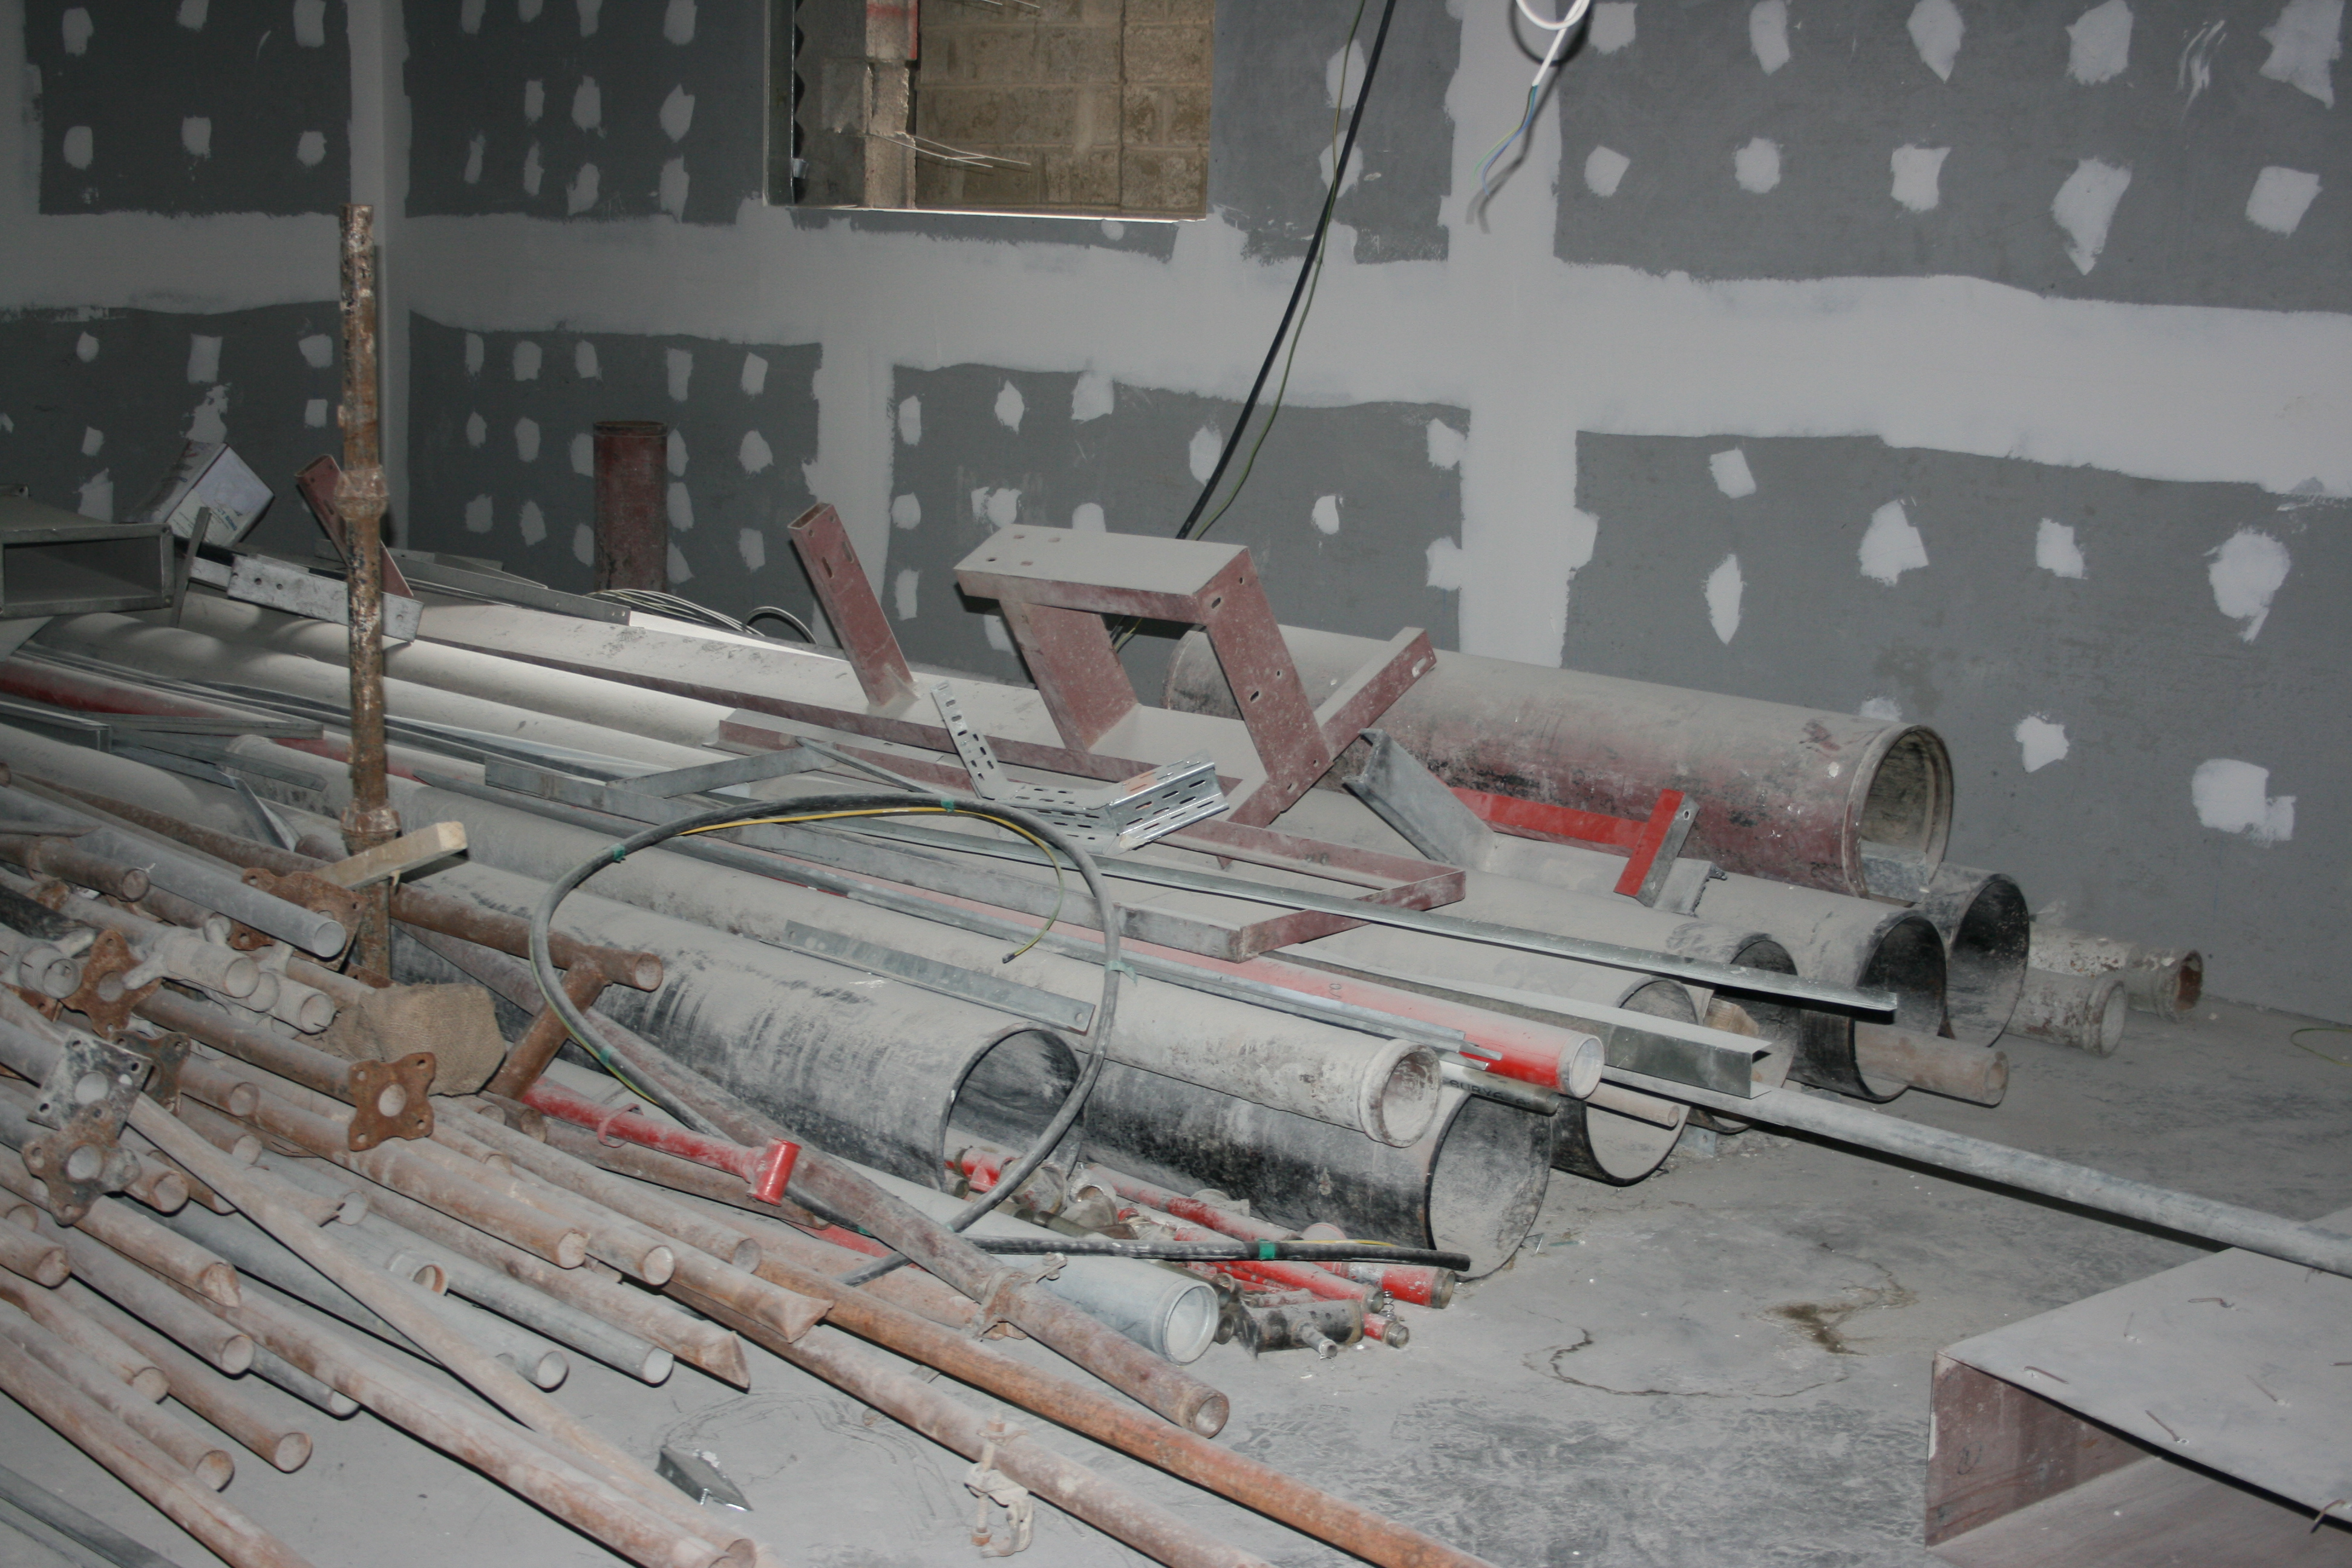
\includegraphics[width=\textwidth]{./graphics/abandoned-materials}
\caption{Abandoned and dirty materials, make for a very unprofessional work place.}
\end{marginfigure}
\section*{Workface Housekeeping}

There is nothing more wasteful than materials and waste lying all over the
place. The section Engineer must set daily procedures and responsibilities
to ensure that all workfaces are clean, even if this entails cleaning
some of the Main Contractor's rubble that was left behind, when they arrived
and made opening that we \textit{forgot} to tell them about. By keeping the
area clean you ensure that not only it is safe to work but waste is
eliminated and productivity improves. Have an adequate supply of clear plastic
bags for the disposal of rubbish (use clear bags to minimize pilferage).


\section*{Protecting the works}
You should ensure that the works are always protected. All piping and ducting should be wrapped in polyethylene when completed and all open ends closed to minimize the amount of debri and dust that can get in. This ensures that
during commissioning less time is spent in cleaning the system. 


\section*{Damage Reports}

However, hard you try at a point you will reach a stage at which some damages
would occur. These are reported properly using a Damages Report format, which
is issued via the Commercial Department as a claim. Be certain that at the
end of the Project you will face the same from other parties. A damaged works
log is to be kept by the QA/QC Department, as well as Document Control.




\section*{Quality}

Although quality assurance and quality control are handled in a dedicated chapter
we have to mention it here. The Section Engineer is resposnible for the quality
of the works in his area. It takes the same effort to complete the works with the right quality as substandard work. In general the following strategy works
well in raising the bar on quality:

\begin{enumerate}
\item Never accept substandard work
\item Prepare a prototype for all works that you are starting for the 
 first time. This will ensure that all stake-holders and technicians understand
the quality of works required.
\item Offer constructive advise to technicians and supervisors during your
Site Walks for work that just does not look right.
\item Snag the works before you  offer them for inspection.
\item Attend the inspections (if not all of them) at least the ones that 
are offered for the first time or that have failed and are offered again for
inspection.
\item Do not offer works for inspection unless you have checked and can verify
that all materials used are as per approved submittals and the installation is as
per approved drawings. Essentially you must make sure that the materials are
correct and the installation is as per the contract, which in most cases is as
per specification and drawings. Investigate any deviations and take remedial
action if necessary.
\end{enumerate}


\begin{marginfigure}
\includegraphics[width=\textwidth]{./graphics/team-spirit}
\caption{Create an environment of openess and co-operation. Quality and targets
are only achieved via a spirit co-operation and Team Work.}
\end{marginfigure}
\subsection*{Quality perception}

Most inspections are \textit{visual} and hence perception psychology plays
an important part. A well lit and \textit{clean} area  with a Team on standby that looks professional, with you having done your homework so that you can answer any question that the
inspector asks will go a long way to a trouble free inspections. With over
30,000 inspections budgeted on larger Projects, if you do not take care of
inspections they are bound to cause delays. 

Other visual items that you will need to take care of is paintwork, supports,
slopes of piping and insulation. 

\begin{marginfigure}
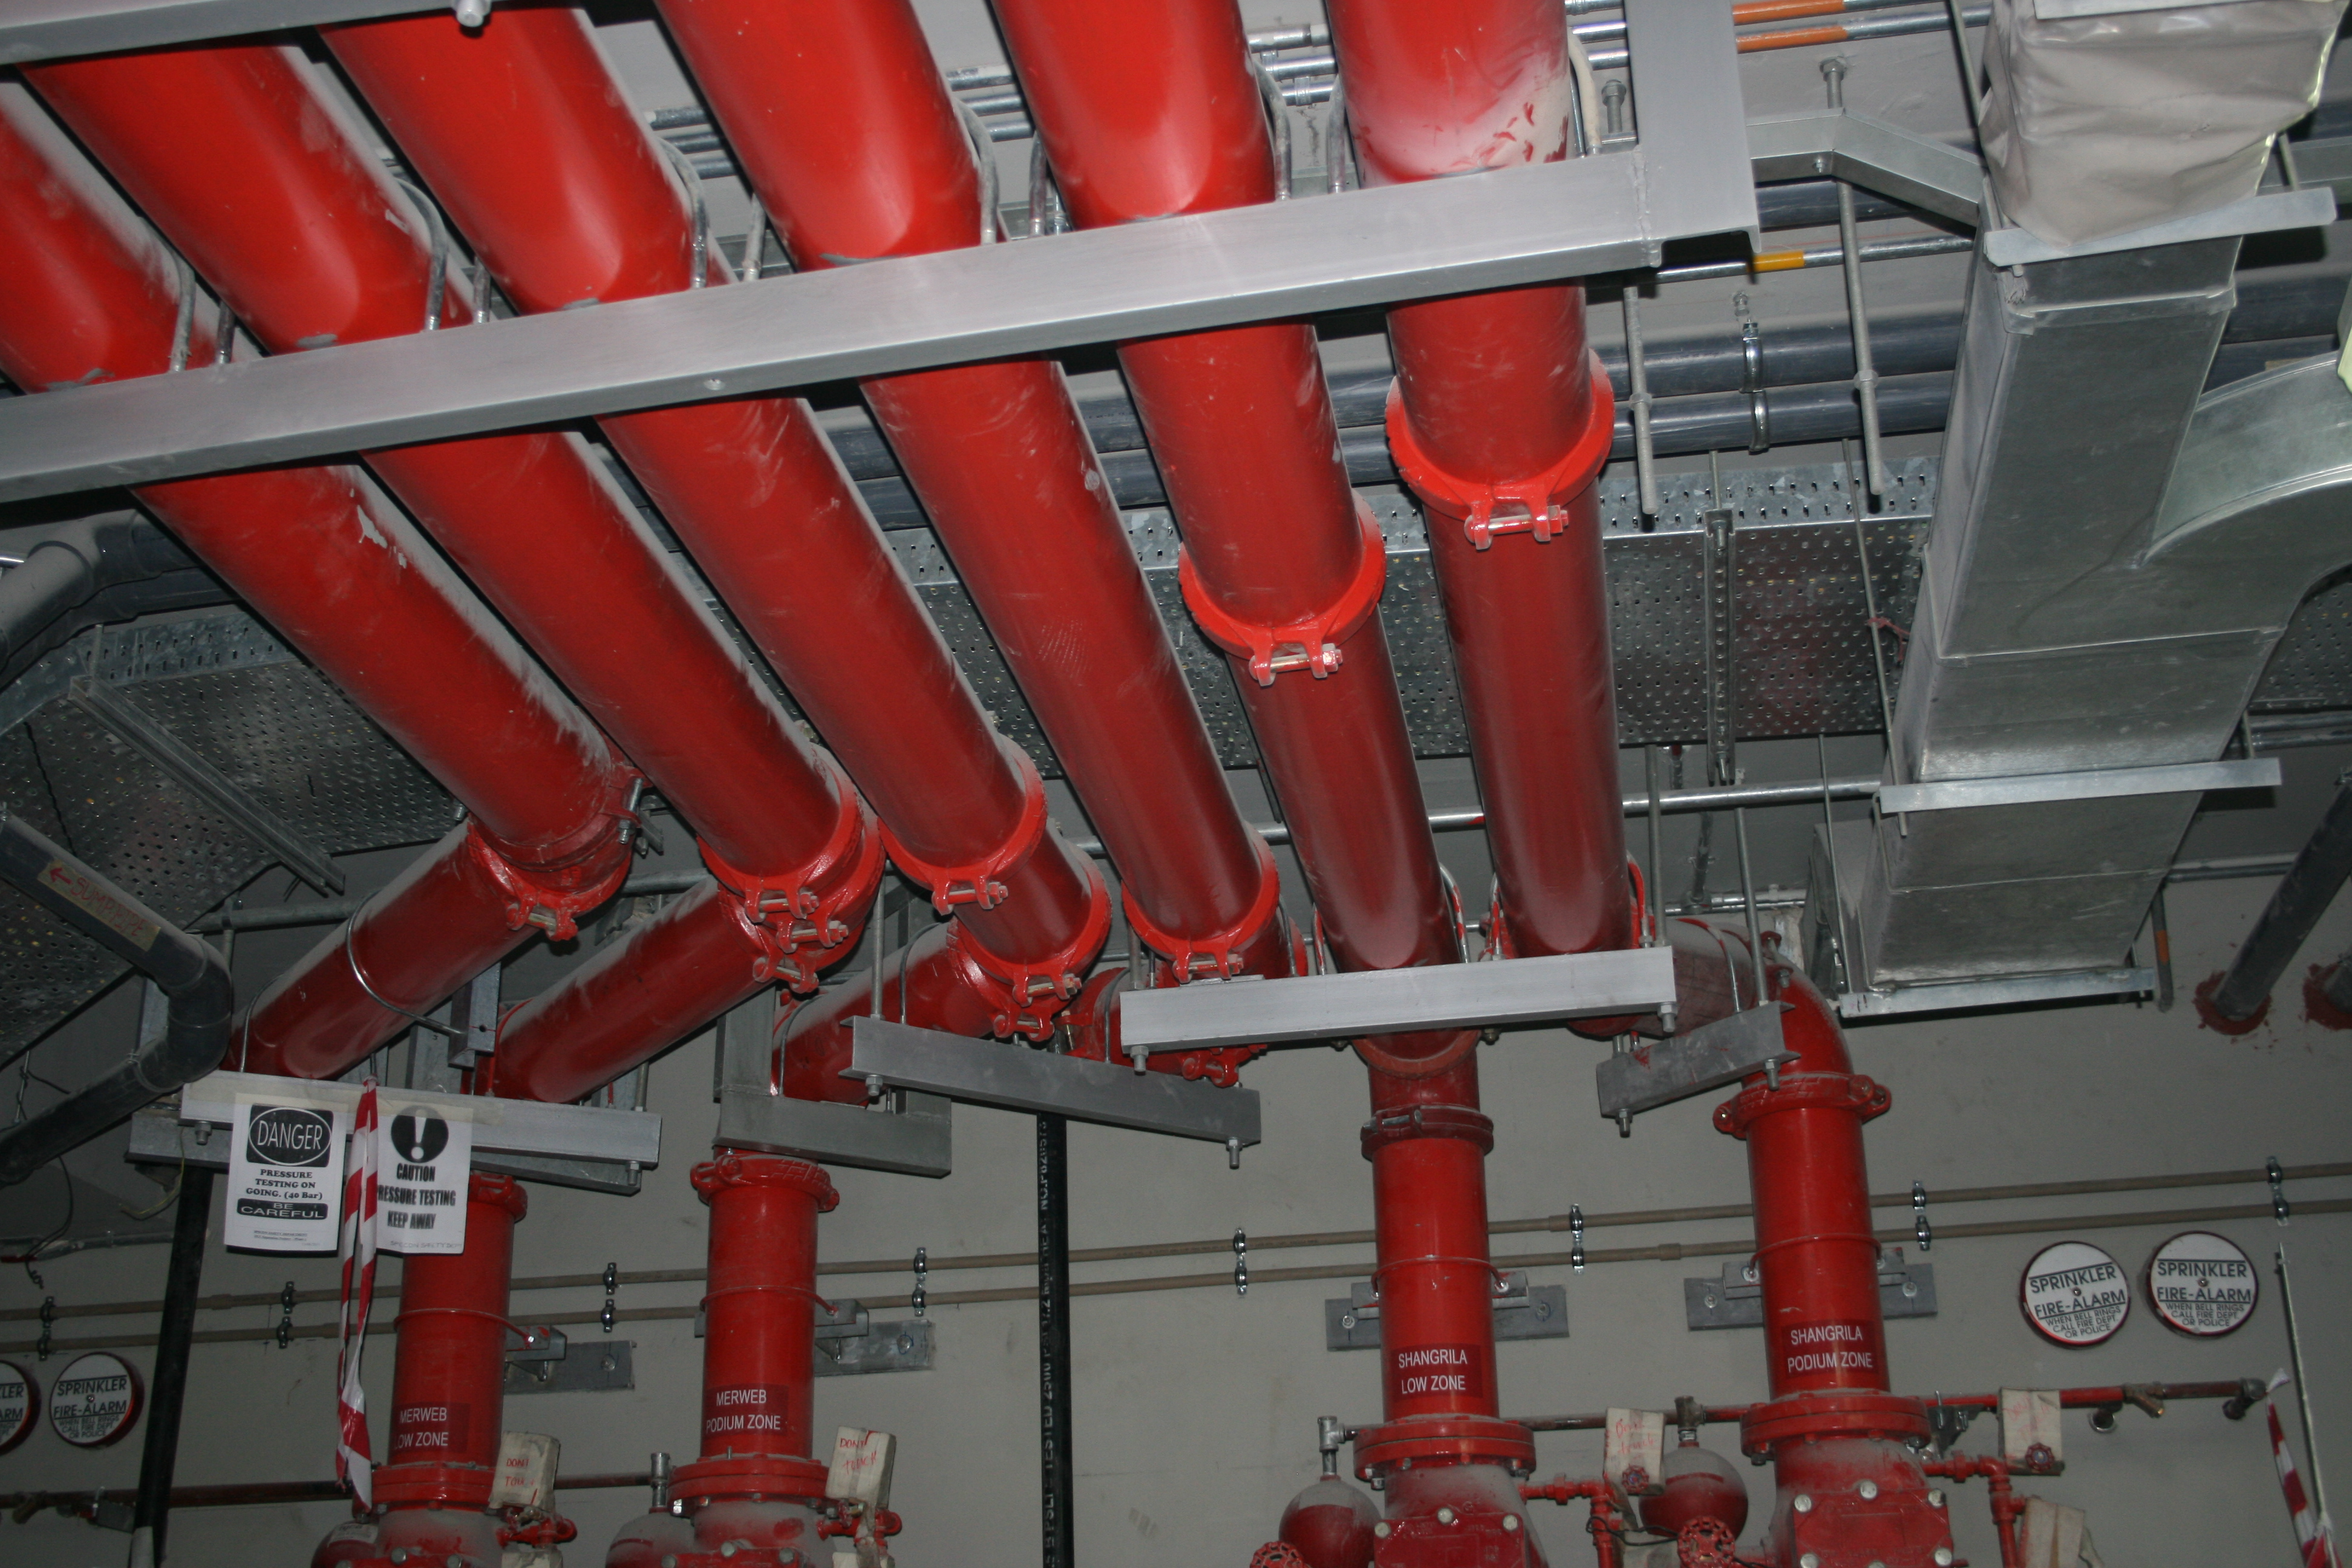
\includegraphics[width=\textwidth]{./graphics/fire-pipes}
\caption{Painted and cleaned piping works and ensuring that nearby pipes run at the same level increase the perception of quality and makes work look professional.}
\end{marginfigure}


\subsection*{Low quality}
If you find that quality is consistently below an acceptable level, make sure 
that you arrange for training for the concerned technicians and or have a prep
talk with everyone. Discuss it with your senior Supervisor and decide what to do.

\section*{Ensure everything will work}

While the daily pressures of work force Engineers to focus on their own section
of works, keep an eye and an enquiry mind to make sure everything works. You 
are the last safety net of both the professional as well as the Contracting Team
to pick up and problems that have not been seen earlier. Ask yourself, will
it work, what happens when something is switched on, can we drain this section
of the works, does it need another valve and so on. You also need to think about
being able to access works for maintenance and also for balancing. So if you have
an access door on a duct taht you cannot open because there is a sprinkler pipe
running across it, you need to take care of it. In general, in this part of the
world, it will cost more to add temporary flushing loops and drains, so ensure
that these have been marked on drawings or take action to request that they are
shown on drawings.



































































